\subsection{Bragg-Reflexion}
Zunächst wird an das aufgenommene Spektrum der unbekannten Anode die Funktion
\begin{align*}
  R(\beta)=a+b\beta+\sum_{i=1}^5 A_i\exp \left(  \frac{-(\beta-\mu_i)^2}{2\sigma_i^2}\right)
\end{align*}
angepasst. Das Ergebnis ist in Abbildung \ref{fig:anode}, die Parameter der Regression in Tabelle \ref{tab:anode} im Anhang zu sehen. 

\begin{figure}[h]
  \centering
  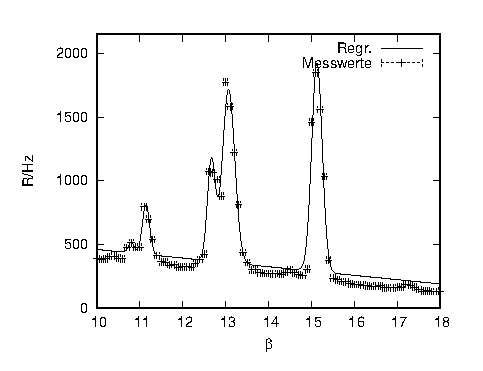
\includegraphics[width=10cm]{data/Bragg/anode.eps}
  \caption{Spektrum der unbekannten Anode unter Bragg-Reflexion}
  \label{fig:anode}
\end{figure}

Für die Bestimmung des Anodenmaterials sind die Schwerpunkte $\mu_i$ relevant. Aus den einzelnen Schwerpunkten können nun über die Bedingung für Interferenzmaxima (siehe Gleichung \ref{eq:bragg}) und den Netzebenenabstand die Wellenlängen und Energien des charakteristischen Spektrums berechnet werden. Für die Berechnung gilt $n=1$, da wir das Spektrum in erster Ordnung aufnehmen. Aus \cite{d_nacl} erhält man den Netzebenenabstand $d=\SI{2,825}{\angstrom}$ für NaCl. Die resultierenden Energien und Wellenlängen sind in Tabelle \ref{tab:spektrum_anode} zu sehen.


Ein Vergleich mit \cite{booklet} zeigt, dass die letzten vier Energien zu dem Spektrum von Wolfram passen. Allerdings liegt kein Literaturwert innerhalb der Fehlergrenzen und alle gemessenen Energien sind größer als der Literaturwert. Dies legt den Schluss nahe, dass es einen Offset in der Winkelmessung gibt. Minimiert man die Summe der Quadrate der Abweichung von Literaturwert und gemessenem Wert folgt für den Offset $\delta \beta=0,068768^\circ$. Die mit dieser Korrektur berechneten Energien sind ebenfalls in Tabelle \ref{tab:spektrum_anode} zu sehen und passen bereits sehr gut zu den Literaturwerten. Trotzdem ist der Literaturwert nicht immer in den Fehlergrenzen. Dies ist nicht verwunderlich, da die Peaks nicht exakt Gaußförmig sind und deshalb auch zu sehen ist, dass die Glockenkurven nicht exakt mittig liegen. Der erste Peak kann nicht dem Spektrum von Wolfram zugeordnet werden. Da die gemessene Zählrate bei dieser Energie deutlich kleiner als die der anderen Energien ist könnte es sich um eine Verunreinigung des Gases handeln. 

\begin{table}[h]
  \centering
  \caption{charakteristisches Spektrum der unbekannten Röhre}
  \label{tab:spektrum_anode}
  \begin{tabular}{c c c c c}
    \toprule
    $i$ & $\lambda/$pm & $E/$keV & $E_\delta/$keV & $E_\mathrm{Lit}/$keV\\
    \midrule
    1   & $106 \pm 1$ & $11,7 \pm 0,1$ & $11,6 \pm 0,6$ & \\
    2   & $109,2 \pm 0,2$ & $11,35 \pm 0,02$ & $11,285 \pm 0,006$ & 11,286\\
    3   & $123,9 \pm 0,1$ & $10,01 \pm 0,01$ & $9,954 \ \pm 0,004$ & 9,962\\
    4   & $127,76 \pm 0,09$ & $\ 9,705 \pm 0,007$ & $9,655 \ \pm 0,004$ & 9,672\\
    5   & $147,44 \pm 0,06$ & $\ 8,409 \pm 0,003$ & $8,372 \ \pm 0,003$ & 8,335\\
    \bottomrule
  \end{tabular}
\end{table}

Das aufgenommene Spektrum der Nachtmessung ist in Abbildung \ref{fig:nachtmessung} zu sehen. Äquivalent zum vorherigen Abschnitt wurde eine Überlagerung aus zwei Glockenkurven und einem Offset an die Messdaten angepasst (Parameter in Tabelle \ref{tab:anode} im Anhang). Die Feinstrukturaufspaltung ist deutlich zu erkennen.

\begin{figure}[h]
  \centering
  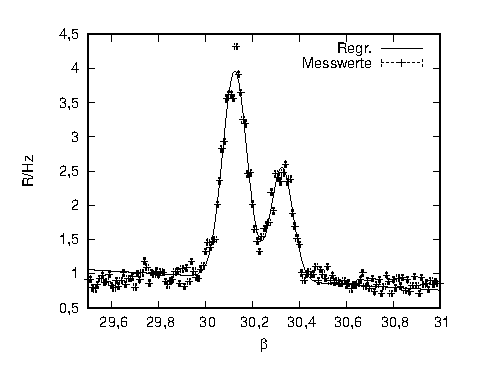
\includegraphics[width=10cm]{data/Bragg/nachtmessung.eps}
  \caption{Feinstrukturaufspaltung von Molybdän}
  \label{fig:nachtmessung}
\end{figure}

Aus den ermittelten Winkeln der Peaks erhält man aus der Bedingung für Interferenzmaxima die Wellenlängen und Energien in Tabelle \ref{tab:nachtmessung}. Hierbei gilt $n=4$, da das Spektrum in vierter Beugungsordnung aufgenommen wurde um die Aufspaltung besser auflösen zu können. Die ermittelten Energien sind beide wieder etwas über dem Literaturwert. Auch hier ist ein Offset eine mögliche Erklärung. Den Wellenlängenunterschied wird der Offset aber kaum beinflussen. Aus den gemessenen Daten erhält man für die Aufspaltung des Dubletts $\Delta \lambda=(0,428 \pm 0,006)$pm. Nach \cite{booklet} liegt die Aufspaltung bei $\Delta \lambda= 0,4287$pm. Der ermittelte Wert passt also sehr gut zum Literaturwert.

\begin{table}[h]
  \centering
  \caption{Feinstrukturaufspaltung von Molybdän}
  \label{tab:nachtmessung}
  \begin{tabular}{c c c c}
    \toprule
    $i$ & $\lambda/$pm & $E/$keV & $E_\mathrm{Lit}/$keV\\
    \midrule
    1   & $70,891 \pm 0,003$ & $17,4894 \pm 0,0006$  & $17,479$\\
    2   & $71,319 \pm 0,005$ & $17,385 \pm 0,001$ &  $17,374$\\
    \bottomrule
  \end{tabular}
\end{table}

\subsection{Analyse chemischer Zusammensetzungen}
An das Spektrum des FeZn-Plättchens wird wie im letzen Kapitel eine Überlagerung aus Glockenkurven angepasst. Diesmal allerdings nur aus vier Glockenkurven, da lediglich drei Peaks direkt sichtbar sind und sich ein vierter, der für die Asymmetrie des ersten Peaks sorgt, vermuten lässt. Das Ergebnis ist in Abbildung \ref{fig:fezn} zu sehen. Offensichtlich wird das Spektrum durch die angenäherte Funktion sehr gut beschrieben. 

\begin{figure}[h]
  \centering
  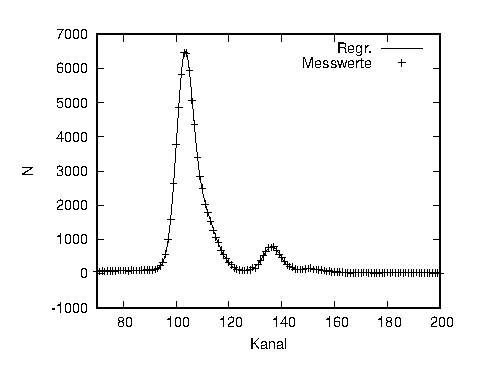
\includegraphics[width=10cm]{data/Massenanteil/fezn.eps}
  \caption{Spektrum des FeZn-Plättchens}
  \label{fig:fezn}
\end{figure}

Aus \cite{booklet} lassen sich die Energien für die vier beobachteten Peaks ermitteln. Die Energie wird gegen den auslösenden Kanal aufgetragen. Eine Regressiongerade $E(N)=a*N+b$ wird angepasst. Das Ergebnis ist in Abbildung \ref{fig:kalibrierung} zu sehen. Bis auf den zweiten Punkt liegt die Gerade im Fehlerbereich aller Punkte. Mit den ermittelten Parametern kann nun jedem Kanal eine Energie zugeordnet werden.

\begin{figure}[h]
  \centering
  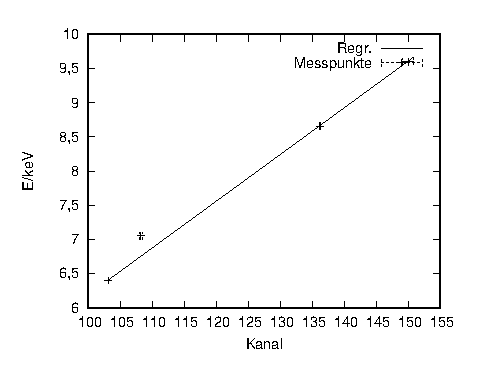
\includegraphics[width=10cm]{data/Massenanteil/kalibrierung.eps}
  \caption{Kalibrierung von Energie zu Kanalnummer}
  \label{fig:kalibrierung}
\end{figure}

Nun kann für alle gemessenen Spektren die Aktivität gegen die Energie aufgetragen werden. Die Parameter befinden sich in Tabelle \ref{tab:parameter_proben} im Anhang, die Graphen am Ende des Abschnitts in Abbildung \ref{fig:proben}.

\paragraph{Probe 1}
Anhand der von Probe 1 emittierten Energien kann auf die chemische Zusammensetzung geschlossen werden. Die erste Emissionslinie $\mu_1=5,41 \pm 0,01$ keV von Probe 1 kann keinem vermessenen Referenzspektrum zugeordnet werden. In \cite{booklet} findet man aber für die $K_\alpha$-Linie von Chrom Energien zwischen 5,415 keV und 5,406 keV (durch Feinstrukturaufspaltung). Somit gehört die erste Emssionslinie von Probe 1 zu Chrom. Die zweite Emissionslinie mit der Energie $\mu_2=6,465 \pm 0,003$ keV kann der ersten Emissionslinie von Eisen mit $6,459 \pm 0,003$ keV zugeordnet werden. Der Vergleich mit dem Spektrum von Eisen zeigt, dass 
\begin{align*}
  \frac{A_2(\mathrm{Probe \ 1})}{A_1(\mathrm{Fe})}=(52,2 \pm 0,6) \%
\end{align*}
der Atome aus Probe 1 Eisenatome sind. Mit den Atommassen von Eisen und Chrom aus \cite{fe} und \cite{cr} erhält man somit die Massenanteile
\begin{align*}
  C_\mathrm{Fe}=(54,0 \pm 0,6) \% \\
  C_\mathrm{Cr}=(46,0 \pm 0,6) \%.
\end{align*}
Bei der Legierung handelt es sich somit um Ferrochrom (siehe \cite{legierung}).

\paragraph{Probe 2 und 3}  Probe 1 emittiert Photonen mit den Energien $\mu_1=(8,048 \pm 0,002)$ keV und $\mu_2= (8,612 \pm 0,006)$ keV. Probe 3 die Energien $\mu_1=(8,041 \pm 0,002)$ keV und $\mu_2=(8,608 \pm 0,005)$ keV. Im Vergleich zu den Referenzspektren passen diese Energien am besten zu $\mu_1$ und $\mu_2$ von Kupfer. In \cite{booklet} findet man für die $K_{\alpha 1}$-Linie von Kupfer eine Energie von 8,048 keV. Diese würde also noch besser zu den Proben passen. Die Diskrepanz zwischen dem Literaturwert und dem gemessenen Wert für Kupfer entsteht unter anderem dadurch, dass die Feinstrukturaufspaltung nicht aufgelöst werden konnte. Die erste Schlussfolgerung wäre also, dass beide Proben nur aus Kupfer bestehen. Diese Angabe ist allerdings mit Vorsicht zu genießen, da die Proben nicht so eindeutig zugeordnet werden konnten wie Probe 1.

\paragraph{Probe 4} Für die letzte Probe wurden die Energien $\mu_1=(5,64 \pm 0,03)$ keV und $\mu_2=(7,021 \pm 0,004)$ keV gemessen. Diese Werte passen zu keinem aufgenommenen Referenzspektrum. In \cite{booklet} findet man für Samarium eine Emissionslinie bei $5,636$ keV und für Eisen eine bei $7,058$ keV. Diese Linien sollten im Spektrum allerdings nicht dominant sein und andere Linien (wie die von uns gemessenen für Eisen) sollten im Spektrum sichtbar sein. Die Zusammensetzung der vierten Probe kann nicht eindeutig bestimmt werden. \\ 

Zusammenfassend konnte nur die Zusammensetzung von Probe 1 bestimmt werden. Bessere Ergebnisse könnten durch die Aufnahme des Spektrums durch Bragg-Reflexion in hoher Ordnung erreicht werden (siehe bestimmte Feinstrukturaufspaltung). Die Messungen würden dann aber auch deutlich mehr Zeit in Anspruch nehmen.

\newpage

\begin{figure}[!h]
  \centering
  \begin{subfigure}[h]{0.5\textwidth}
    \centering
    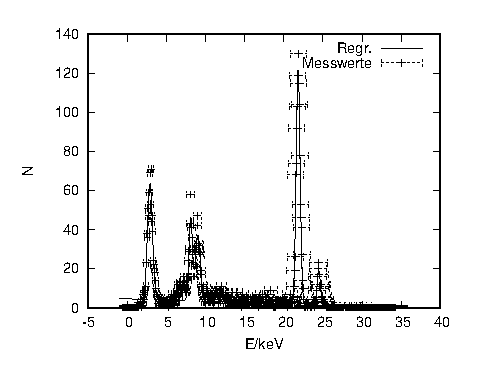
\includegraphics{data/Massenanteil/ag.eps}
    \subcaption{Ag}
  \end{subfigure}%
  \begin{subfigure}[h]{0.5\textwidth}
    \centering
    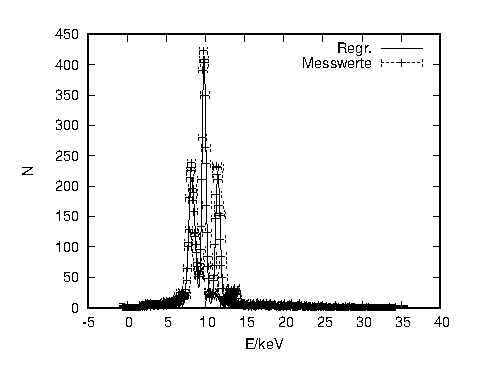
\includegraphics{data/Massenanteil/au.eps}
    \subcaption{Au}
  \end{subfigure}
  \begin{subfigure}[h]{0.5\textwidth}
    \centering
    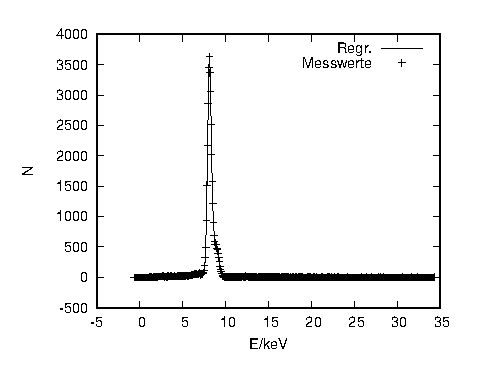
\includegraphics{data/Massenanteil/cu.eps}
    \subcaption{Cu}
  \end{subfigure}%
  \begin{subfigure}[h]{0.5\textwidth}
    \centering
    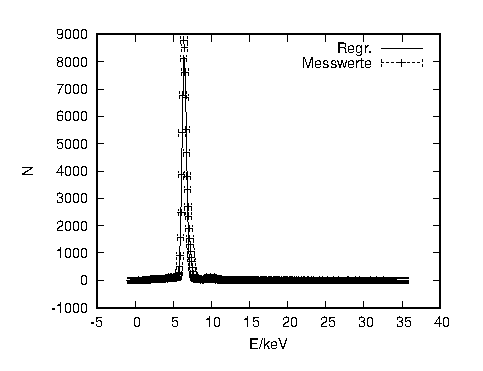
\includegraphics{data/Massenanteil/fe.eps}
    \subcaption{Fe}
  \end{subfigure}
  \begin{subfigure}[h]{0.5\textwidth}
    \centering
    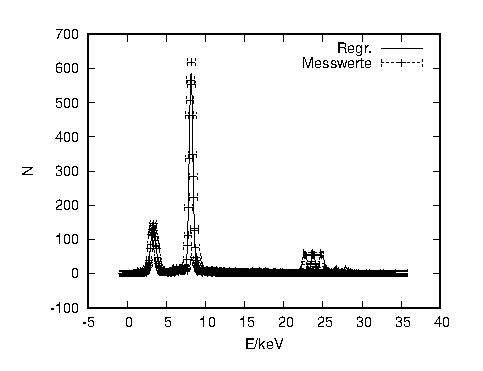
\includegraphics{data/Massenanteil/in.eps}
    \subcaption{In}
  \end{subfigure}%
  \begin{subfigure}[h]{0.5\textwidth}
    \centering
    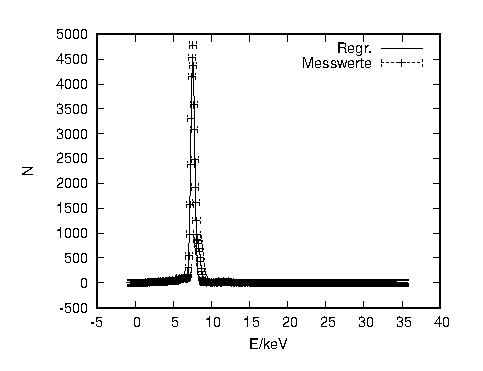
\includegraphics{data/Massenanteil/ni.eps}
    \subcaption{Ni}
  \end{subfigure}
\end{figure}

\newpage

\begin{figure}[!h]
  \ContinuedFloat
  \centering
  \begin{subfigure}[h]{0.5\textwidth}
    \centering
    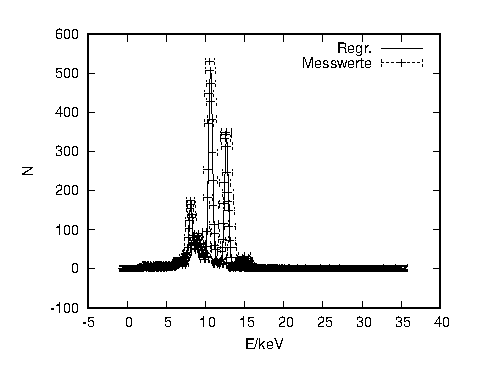
\includegraphics{data/Massenanteil/pb.eps}
    \subcaption{Pb}
  \end{subfigure}%
  \begin{subfigure}[h]{0.5\textwidth}
    \centering
    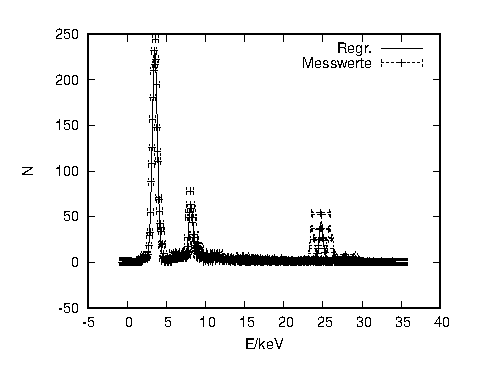
\includegraphics{data/Massenanteil/sn.eps}
    \subcaption{Sn}
  \end{subfigure}
  \begin{subfigure}[h]{0.5\textwidth}
    \centering
    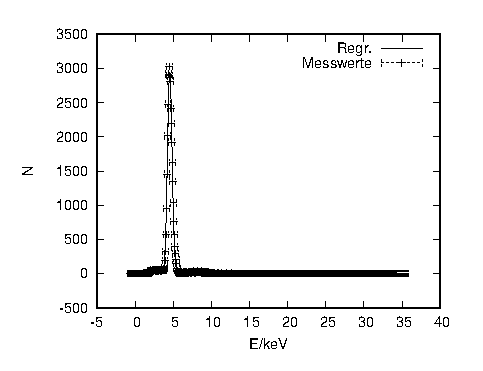
\includegraphics{data/Massenanteil/ti.eps}
    \subcaption{Ti}
  \end{subfigure}%
  \begin{subfigure}[h]{0.5\textwidth}
    \centering
    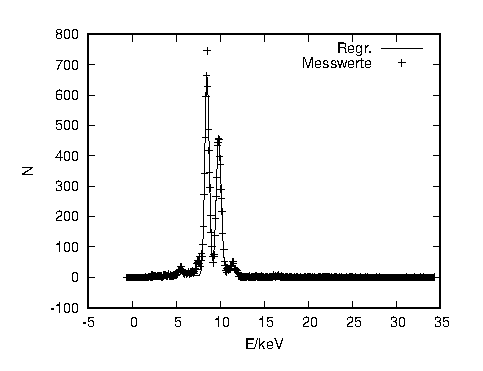
\includegraphics{data/Massenanteil/w.eps}
    \subcaption{W}
  \end{subfigure}
  \begin{subfigure}[h]{0.5\textwidth}
    \centering
    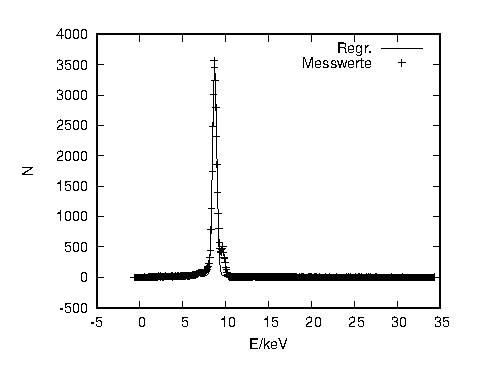
\includegraphics{data/Massenanteil/zn.eps}
    \subcaption{Zn}
  \end{subfigure}%
  \begin{subfigure}[h]{0.5\textwidth}
    \centering
    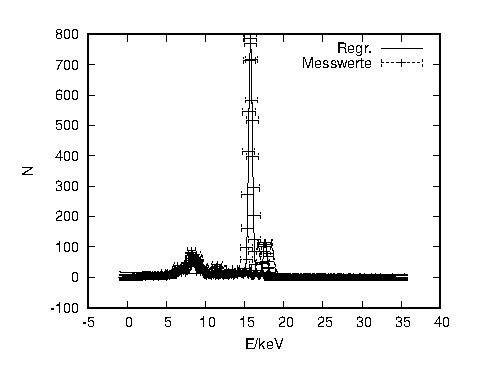
\includegraphics{data/Massenanteil/zr.eps}
    \subcaption{Zr}
  \end{subfigure}
\end{figure}

\newpage

\begin{figure}[!h]
  \ContinuedFloat
  \centering
  \begin{subfigure}[h]{0.5\textwidth}
    \centering
    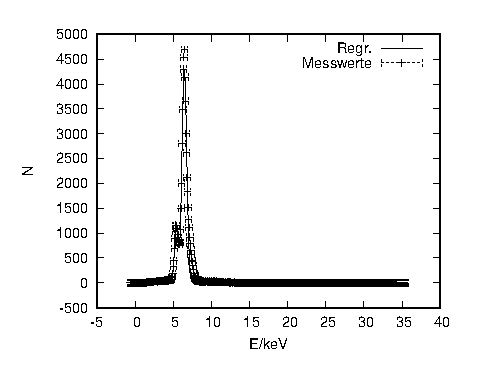
\includegraphics{data/Massenanteil/probe_1.eps}
    \subcaption{Probe 1}
  \end{subfigure}%
  \begin{subfigure}[h]{0.5\textwidth}
    \centering
    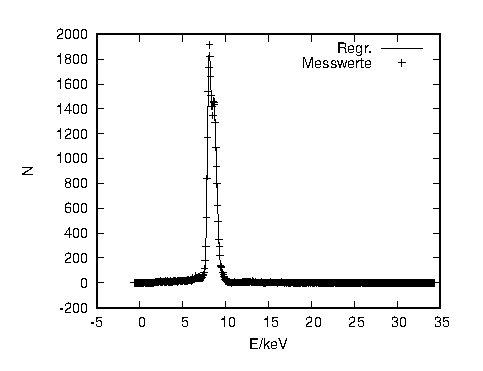
\includegraphics{data/Massenanteil/probe_2.eps}
    \subcaption{Probe 2}
  \end{subfigure}
  \begin{subfigure}[h]{0.5\textwidth}
    \centering
    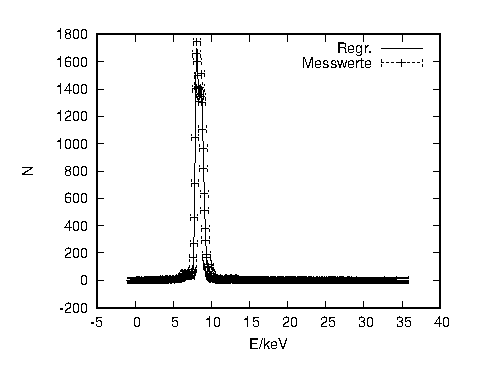
\includegraphics{data/Massenanteil/probe_3.eps}
    \subcaption{Probe 3}
  \end{subfigure}%
  \begin{subfigure}[h]{0.5\textwidth}
    \centering
    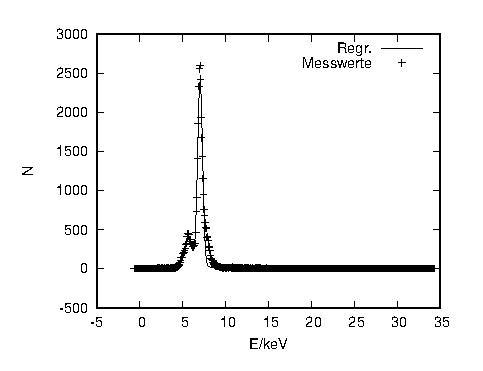
\includegraphics{data/Massenanteil/probe_4.eps}
    \subcaption{Probe 4}
  \end{subfigure}
  \caption{Aufgenommene Spektren für verschiedene Proben}
  \label{fig:proben}
\end{figure}
